%!TEX root = main.tex

Suponga que una fuente genera la secuencia típica aabbcccaadeeeaabcaadcdabbedededecacaeeddcccodcdeaabedbb. Determine un par de códigos Tunstall sobre alfabetos binarios y triarios, indique los diccionarios en cada caso. Cuál de los códigos trabajaría más eficiente?
\begin{sols}
 Como nos dan una secuencia típica, realicemos la tabla de frecuencias para determinar la probabilidad de cada símbolo:
 \begin{center}
  \begin{tabular}{|c|c|c|}
  \hline
Simbolo & Frecuencia & Probabilidad \\
\hline
$a$ & $13$ & $13/55$\\
\hline
$b$ & $8$ & $8/55$\\
\hline
$c$ & $12$ & $12/55$\\
\hline
$d$ & $11$ & $11/55$\\
\hline
$e$ & $11$ & $11/55$\\
\hline
 \end{tabular}
 \end{center}
Con esta información podemos proceder con cada código de Tunstall.\\

\textbf{Sobre un alfabeto Binario:}\\

Consideramos $D_z=2$ y $D_u=5.$ Seguiremos por pasos el algoritmo:

\textbf{Paso 1:}
\begin{itemize}
    \item[a)] Queremos un $n$, tal que $2^n\geq 5$, por lo que escogeremos $n=3$, ya que es el primer natural que lo cumple, esta sera nuestra longitud de palabra.
    \item[b)] Tenemos que $k=\left\lfloor\dfrac{2^3-1}{5-1}\right\rfloor=\left\lfloor\dfrac{7}{4}\right\rfloor=1.$ Dado que este es el numero de nodos internos, podemos inferir en este paso que solo tendremos a la raíz como nodo interno.
    \item[c)] Por lo anterior tenemos que $M=1+1(5-1)=5.$ Es decir que el numero de mensajes a codificar es el mismo que el de símbolos de la fuente.
\end{itemize}
\textbf{Paso 2:}
 Note que en este paso del algoritmo como resaltamos antes solo asignamos hijos a la raíz, cuando hacemos $j=1$, ya que $k=1.$ Por  lo que el árbol construido es el siguiente:
 \begin{center}
       \begin{tikzpicture}

            \node[solid, label=above:{1}](0){}
                child{node[solid, label=below:{$\dfrac{13}{55}$}]{}  edge from parent node[above]{$a$}}
                child{node[solid, label=below:{$\dfrac{8}{55}$}]{}  edge from parent node[left]{$b$}}
                child{node[solid, label=below:{$\dfrac{12}{55}$}]{}  edge from parent node[left]{$c$}}
                child{node[solid, label=below:{$\dfrac{11}{55}$}]{}  edge from parent node[left]{$d$}}
                child{node[solid, label=below:{$\dfrac{11}{55}$}]{}  edge from parent node[above]{$e$}}
;
\end{tikzpicture}
    \end{center}
De esta manera un diccionario de codificación para el caso binario es el siguiente
\begin{center}
  \begin{tabular}{|c|c|c|c|c|}
  \hline
$a$ & $b$ & $c$ & $d$ & $e$\\
\hline
$000$ & $001$ & $010$ & $011$ & $100$\\
\hline
 \end{tabular}
 \end{center}

Ahora para calcular la eficiencia sabemos que $\overline{L}_z=3$, ya que el código tiene esa longitud constante. La entropía de nuestra fuente esta dada por
\begin{align*}
    H_2(F)&=-\dfrac{13}{55}\log_2\dfrac{13}{55}-\dfrac{8}{55}\log_2\dfrac{8}{55}-\dfrac{12}{55}\log_2\dfrac{12}{55}-\dfrac{11}{55}\log_2\dfrac{11}{55}-\dfrac{11}{55}\log_2\dfrac{11}{55}\\
    &\approx2.3044.
\end{align*}
Por ultimo hallamos la longitud promedio de mensaje emitido
\begin{align*}
   \overline{L}_u&=\dfrac{13}{55}\cdot1+\dfrac{8}{55}\cdot1+\dfrac{12}{55}\cdot1+\dfrac{11}{55}\cdot1+\dfrac{11}{55}\cdot1\\
   &=1. 
\end{align*}
Note que esto tiene sentido ya que los mensajes son todos de longitud 1. Luego tenemos que la eficiencia para este código es
$$\eta_2=\dfrac{H_2(F)\overline{L}_u}{\overline{L}_z}\approx\dfrac{2.3044}{3}\approx0.76813\approx 76\%.$$



\textbf{Sobre un alfabeto Triario:}\\

Consideramos $D_z=3$ y $D_u=5.$ Nuevamente seguiremos el algoritmos:

\textbf{Paso 1:}
\begin{itemize}
    \item[a)] Queremos un $n$, tal que $3^n\geq 5$, por lo que escogeremos $n=2$, ya que es el primer natural que lo cumple, esta sera nuestra longitud de palabra.
    \item[b)] Tenemos que $k=\left\lfloor\dfrac{3^2-1}{5-1}\right\rfloor=\left\lfloor\dfrac{8}{4}\right\rfloor=2.$ Este sera el numero de nodos internos.
    \item[c)] Por lo anterior tenemos que $M=1+2(5-1)=9.$ Este sera el numero de mensajes a codificar.
\end{itemize}
\textbf{Paso 2:}
Al igual que en el caso anterior para el paso $j=1$, tenemos el siguiente árbol

\begin{center}
       \begin{tikzpicture}
            \node[solid, label=above:{1}](0){}
                child{node[solid, label=below:{$\dfrac{13}{55}$}]{}  edge from parent node[above]{$a$}}
                child{node[solid, label=below:{$\dfrac{8}{55}$}]{}  edge from parent node[left]{$b$}}
                child{node[solid, label=below:{$\dfrac{12}{55}$}]{}  edge from parent node[left]{$c$}}
                child{node[solid, label=below:{$\dfrac{11}{55}$}]{}  edge from parent node[left]{$d$}}
                child{node[solid, label=below:{$\dfrac{11}{55}$}]{}  edge from parent node[above]{$e$}}
;
\end{tikzpicture}
    \end{center}
Para el paso $j=2$, como $k=2$, por el algoritmo esta es la ultima iteración. Como tenemos que tomar el nodo de mayor probabilidad, tomamos el de la rama de $a$, por lo que el árbol que nos da la codificación es el siguiente
\begin{center}
       \begin{tikzpicture}[level 1/.style={level distance=15mm, sibling distance=20mm}, level 2/.style={level distance=35mm}]
            \node[solid, label=above:{1}](0){}
                child{node[solid, label=above:{$\dfrac{13}{55}$}]{}
                    child{node[solid, label=below:{$\dfrac{169}{3025}$}]{}  edge from parent node[above]{$a$}}
                    child{node[solid, label=below:{$\dfrac{104}{3025}$}]{}  edge from parent node[left]{$b$}}
                    child{node[solid, label=below:{$\dfrac{156}{3025}$}]{}  edge from parent node[left]{$c$}}
                    child{node[solid, label=below:{$\dfrac{143}{3025}$}]{}  edge from parent node[left]{$d$}}
                    child{node[solid, label=below:{$\dfrac{143}{3025}$}]{}  edge from parent node[above]{$e$}}
                      edge from parent node[above]{$a$}}
                child{node[solid, label=below:{$\dfrac{8}{55}$}]{}  edge from parent node[left]{$b$}}
                child{node[solid, label=below:{$\dfrac{12}{55}$}]{}  edge from parent node[left]{$c$}}
                child{node[solid, label=below:{$\dfrac{11}{55}$}]{}  edge from parent node[left]{$d$}}
                child{node[solid, label=below:{$\dfrac{11}{55}$}]{}  edge from parent node[above]{$e$}}
;
\end{tikzpicture}
    \end{center}
Con esto en mente el diccionario de codificación para el caso triario es el siguiente
\begin{center}
  \begin{tabular}{|c|c|c|c|c|c|c|c|c|}
  \hline
$aa$ & $ab$ & $ac$ & $ad$ & $ae$ & $b$ & $c$ & $d$ & $e$\\
\hline
$00$ & $01$ & $02$ & $10$ & $11$ & $12$ & $20$ & $21$ & $22$\\
\hline
 \end{tabular}
 \end{center}
Para la eficiencia en este caso tenemos que $\overline{L}_z=2$, mientras que la entropía para este caso como estamos en un código triario es de la forma
$$H_3(F)=\dfrac{H_2(F)}{log_2(3)}\approx1.45391.$$
Luego falta con calcular la longitud promedio de mensaje, que esta dada por
\begin{align*}
    \overline{L}_u&=2\cdot\left(\dfrac{169}{3025}+\dfrac{104}{3025}+\dfrac{156}{3025}+\dfrac{143}{3025}+\dfrac{143}{3025}\right)+\dfrac{8}{55}\cdot1+\dfrac{12}{55}\cdot1+\dfrac{11}{55}\cdot1+\dfrac{11}{55}\cdot1\\
    &=\dfrac{26}{55}\cdot1+\dfrac{8}{55}\cdot1+\dfrac{12}{55}\cdot1+\dfrac{11}{55}\cdot1+\dfrac{11}{55}\cdot1\\
   &=\dfrac{68}{55}. 
\end{align*}
Luego tenemos que la eficiencia en el caso triario esta dado por
$$\eta_3=\dfrac{H_3(F)\overline{L}_u}{\overline{L}_z}\approx\dfrac{(1.45391)\left(\dfrac{68}{55}\right)}{2}\approx 0.89778\approx 89\%$$

De esta manera como $\eta_2<\eta_3,$ concluimos que es mas eficiente el código triario. esto era esperable ya que en el caso binario estábamos codificando símbolo a símbolo de la fuente.
\end{sols}